\documentclass[12pt,a4paper]{article}
\usepackage[T1]{fontenc}
\usepackage[utf8]{inputenc}
\usepackage{mathptmx}
% the symbols of mathptmx need the rsfs font, which is not installed: symbols from Computer Modern
\DeclareSymbolFont{symbols}{OMS}{cmsy}{m}{n}
\usepackage{textcomp}
\usepackage[a4paper,margin=25mm]{geometry}
\usepackage{graphicx}
\usepackage{booktabs}
\usepackage{tabularx}
\usepackage{amsmath}
\usepackage{url}
\usepackage[hidelinks]{hyperref}
\urlstyle{same}

\graphicspath{{figs/}}
\linespread{1.1}
\setlength{\parindent}{1.5em}
\setlength{\parskip}{0pt}
\clubpenalty=10000
\widowpenalty=10000
\displaywidowpenalty=10000
\renewcommand{\topfraction}{0.9}
\renewcommand{\bottomfraction}{0.6}
\renewcommand{\textfraction}{0.08}
\renewcommand{\floatpagefraction}{0.9}
\setcounter{topnumber}{2}
\setcounter{totalnumber}{3}
\hypersetup{pdftitle={The whole f-I curve of a neuron from its rheobase and one current step},
  pdfauthor={Mikhail Smirnov}}

\makeatletter
% captions: small type, bold label, one size for all figures and tables
\long\def\@makecaption#1#2{\vskip\abovecaptionskip{\small\textbf{#1.}\ #2\par}\vskip\belowcaptionskip}
\renewcommand\section{\@startsection{section}{1}{\z@}{-3.0ex \@plus -1ex \@minus -.2ex}{1.2ex \@plus .2ex}{\normalfont\large\bfseries}}
\renewcommand\subsection{\@startsection{subsection}{2}{\z@}{-2.2ex \@plus -.6ex \@minus -.2ex}{0.6ex \@plus .1ex}{\normalfont\normalsize\itshape}}
\makeatother
\setlength{\abovecaptionskip}{6pt}

\newcommand{\Irh}{I_{\mathrm{rh}}}
\newcommand{\taum}{\tau_{\mathrm{m}}}
\newcommand{\lgt}{\log_{10}}

\begin{document}

\begin{flushleft}
{\LARGE\bfseries The whole f--I curve of a neuron from its rheobase and one current step: a pre-registered test of a one-parameter logarithmic law on the Allen Cell Types Database\par}
\vspace{12pt}
{\large Mikhail Smirnov\par}
\vspace{3pt}
{\small Independent researcher, Valencia, Spain\\
\href{mailto:lab@mindscan.org}{lab@mindscan.org} \quad ORCID: \href{https://orcid.org/0009-0000-2251-6698}{0009-0000-2251-6698}\\
DOI:\href{https://doi.org/10.5281/zenodo.23582787}{10.5281/zenodo.23582787}\par}
\end{flushleft}
\vspace{6pt}

\noindent\rule{\textwidth}{0.4pt}
\vspace{2pt}

\noindent\textbf{Abstract.} The frequency--current (f--I) curve of a neuron is usually summarised by the slope of a straight line above the rheobase, or by a fitted neuron model. I tested a one-parameter law, $f = k\ln(I/\Irh)$, where $\Irh$ is the rheobase, on 2,333 mouse and human neurons of the Allen Cell Types Database (58,585 one-second current steps). The hypotheses, the data split and the error measure were fixed and fingerprinted before a single look at 700 held-out cells. The error of a predicted rate is $|\lgt(f_{\mathrm{pred}}/f)|$, in decades. On the 588 held-out cells with at least seven suprathreshold steps, calibrating $k$ from the rheobase and one step near $2\Irh$ predicts the rest of the curve with a median error of 0.084 decades (a factor of 1.21), against 0.120 decades (1.32) for a straight line through the same two points. Fitted to the lowest 60\,\% of a cell's steps, the two-parameter form $a + b\ln(I/\Irh)$ predicts the remaining, higher steps with a median error of 0.054 decades, against 0.074 for a straight line. The zero of the fitted logarithm lies at the rheobase (median $I_0/\Irh = 0.987$). Outside the registration, on the 331 held-out cells with published generalized leaky integrate-and-fire models (GLIF3), the cells' own models predicted the rates with a median error of 0.200 decades, against 0.078 for the one-step law, and $k$ scaled close to $1/\taum$. The law is a practical compromise rather than the exact shape of every cell: with typically 7 to 10 steps per cell, both the logarithm and the straight line are consistent with the count noise for most cells.

\vspace{4pt}
\noindent\textbf{Keywords:} f--I curve; rheobase; firing rate; neuronal gain; Allen Cell Types Database; pre-registration

\vspace{2pt}
\noindent\rule{\textwidth}{0.4pt}

\section{Introduction}

The f--I curve, the firing rate of a neuron as a function of an injected current, is among the most often measured properties of a neuron. It enters cell-type classification (Gouwens et al.\ 2019), it sets the gain of point-neuron models (Teeter et al.\ 2018), and its nonlinearity shapes the distribution of firing rates in networks (Roxin et al.\ 2011). Since Hodgkin (1948), curves have been sorted into those that rise continuously from zero at threshold and those that jump to a finite rate. Fits used in practice include a straight line above the rheobase (the summary the Allen Cell Types Database itself reports), expansive power laws at low rates, where input fluctuations smooth the threshold (Roxin et al.\ 2011), and the power function $f = (aI - b)^d$ (Tateno et al.\ 2004), which becomes strongly sublinear as $d$ approaches zero.

This note asks a practical question: how much of a cell's f--I curve can be recovered from the fewest measurements? I tested a one-parameter logarithmic law anchored at the rheobase,
\[ f = k\ln(I/\Irh), \]
on a large public dataset, with a pre-registered held-out test. The logarithm is the $d \to 0$ limit of the power family, $(x^d - 1)/d \to \ln x$, so it is not a new functional form. What is tested is whether its one-parameter version, with its zero fixed at the rheobase, is a useful predictor across many cell types, and how it compares with a straight line and with the database's own neuron models.

\section{Data and methods}

\subsection{Data}
I used the Allen Cell Types Database (Allen Institute for Brain Science), downloaded through its public API on 22 October 2026: 2,333 cells (mouse and human) and 58,585 Long Square sweeps, that is, one-second steps of constant current. For each cell and each current at or above the cell's rheobase (the database's feature \texttt{threshold\_i\_long\_square}) that produced spikes, the rate $f$ is the number of spikes per second, averaged over repeated steps of the same amplitude, and $x = I/\Irh$. Currents at or above the rheobase that produced no spike (411 of 19,047, in 298 cells) were left out. Cells with at least seven such points enter the checks below; for 96\,\% of them the first point is the step at the rheobase itself ($x = 1$). The cells have a median of 8 points (10th to 90th percentile: 7 to 10).

\subsection{Split and registration}
Before any analysis, 30\,\% of the cells (700, random seed 20261022) were set aside as the test. Exploration used only the remaining 1,633 cells (the working part), in two independent internal splits that each set aside 30\,\% of them for checking; it compared 15 variants of the set-up (targets $f$ and $\lgt f$, limits on the constants, forms of the law for $k$). The hypotheses below, the scripts, the expected outcomes from the exploration, and the SHA-256 digests of the downloaded data and of the formula-search program were recorded in a registration document. Its SHA-256 fingerprint,
\begin{center}\small\texttt{cd36fae6e1542abacfd38bde0ea0acefa4b86eb735f2d786d4941c70a7961cc2},\end{center}
was taken on 22 October 2026 at 16:20~UTC, before the test cells were read. The test was then read once, and no deviation from the protocol was needed.

\subsection{Checks}
The error of a predicted rate is $|\lgt(f_{\mathrm{pred}}/f)|$, in decades (0.1 decades is a factor of 1.26), with predictions below 0.5~Hz counted as 0.5~Hz. Errors are pooled over the steps of all cells.

\textit{(A) Continuation.} Per-cell forms are fitted by least squares to the cell's lowest 60\,\% of steps (at least three) and predict its remaining, higher steps.

\textit{(B) One-step calibration.} $k = f_1/\ln x_1$ is taken from the step nearest $x = 2$ among those with $x > 1.2$, and predicts every other step of the cell, the rheobase step included. The comparison is the straight line through the threshold and the same step, $f_1(x - 1)/(x_1 - 1)$. At the rheobase both predictions are zero and are counted as 0.5~Hz.

\textit{(C) The zero of the law.} $x_0 = \exp(-a/b)$ of $a + b\ln x$ fitted to the cell's whole curve, for the cells with $b > 0$.

\textit{(D) $k$ from the cell's properties.} For every cell, $k$ is the least-squares fit of $k\ln x$ to its whole curve. $\lgt k$ is predicted from the membrane time constant $\taum$, the input resistance $R$, the rheobase, the dendrite type and the species, by a law fitted on the 1,340 working-part cells with at least seven steps and applied to the held-out cells.

\subsection{Registered hypotheses}
H1: in (A), $a + b\ln x$ has a lower mean and a lower median error than the line $a + bx$. H2: in (B), the median error of $k\ln x$ is below 0.85 times that of the line through the threshold. H3: in (C), the median $x_0$ lies between 0.93 and 1.03. H4: in (D), a law found by the formula-search program NAI predicts $\lgt k$ with a lower mean absolute error than a log-linear least-squares regression on the same properties.

\subsection{Formula search}
The logarithmic family and the law for $k$ were found during exploration with NAI (Smirnov, version 21), a symbolic-regression program I develop, which searches for formulas without a given form and uses no language model. Searching one form for many cells at once, with numbers fitted per cell, it returned forms such as $a + b\ln(x - c)$; the one-parameter form $k\ln x$ is my simplification of them. For check D, NAI (version 21) searched for 300~s with a fixed random seed; the program and its settings are fixed by the registration.

\subsection{GLIF models (outside the registration)}
Of the 2,333 cells, 1,218 have published GLIF1 (leaky integrate-and-fire) and GLIF3 (with after-spike currents) models (Teeter et al.\ 2018); 1,086 of them have at least seven steps (755 in the working part, 331 held out, of which 285 are mouse and 46 human cells). I simulated each model on the cell's own current amplitudes with the published parameters and equations: forward Euler with the models' time step of 50~\textmu s, reset of the voltage to rest, the after-spike currents added at each spike, and the voltage held for the published refractory period after a spike. The simulation is my re-implementation; for GLIF1 it agrees with the analytic rate of a leaky integrate-and-fire neuron.

\section{Results}

\subsection{Registered checks}
All four hypotheses held (Table~\ref{tab:checks}). Among the other registered forms of check A (Table~\ref{tab:forms}), two of the three forms with three numbers per cell, $a + b\ln(x - c)$ and the saturating exponential $a - b\exp(-x/c)$, were as accurate as $a + b\ln x$; the shifted power law $a + b(x - 1)^p$ and the square root were less accurate. The logarithm's advantage is that one number per cell loses little. Figure~\ref{fig:curves} shows six held-out cells.

\begin{figure}[tbp]
\centering
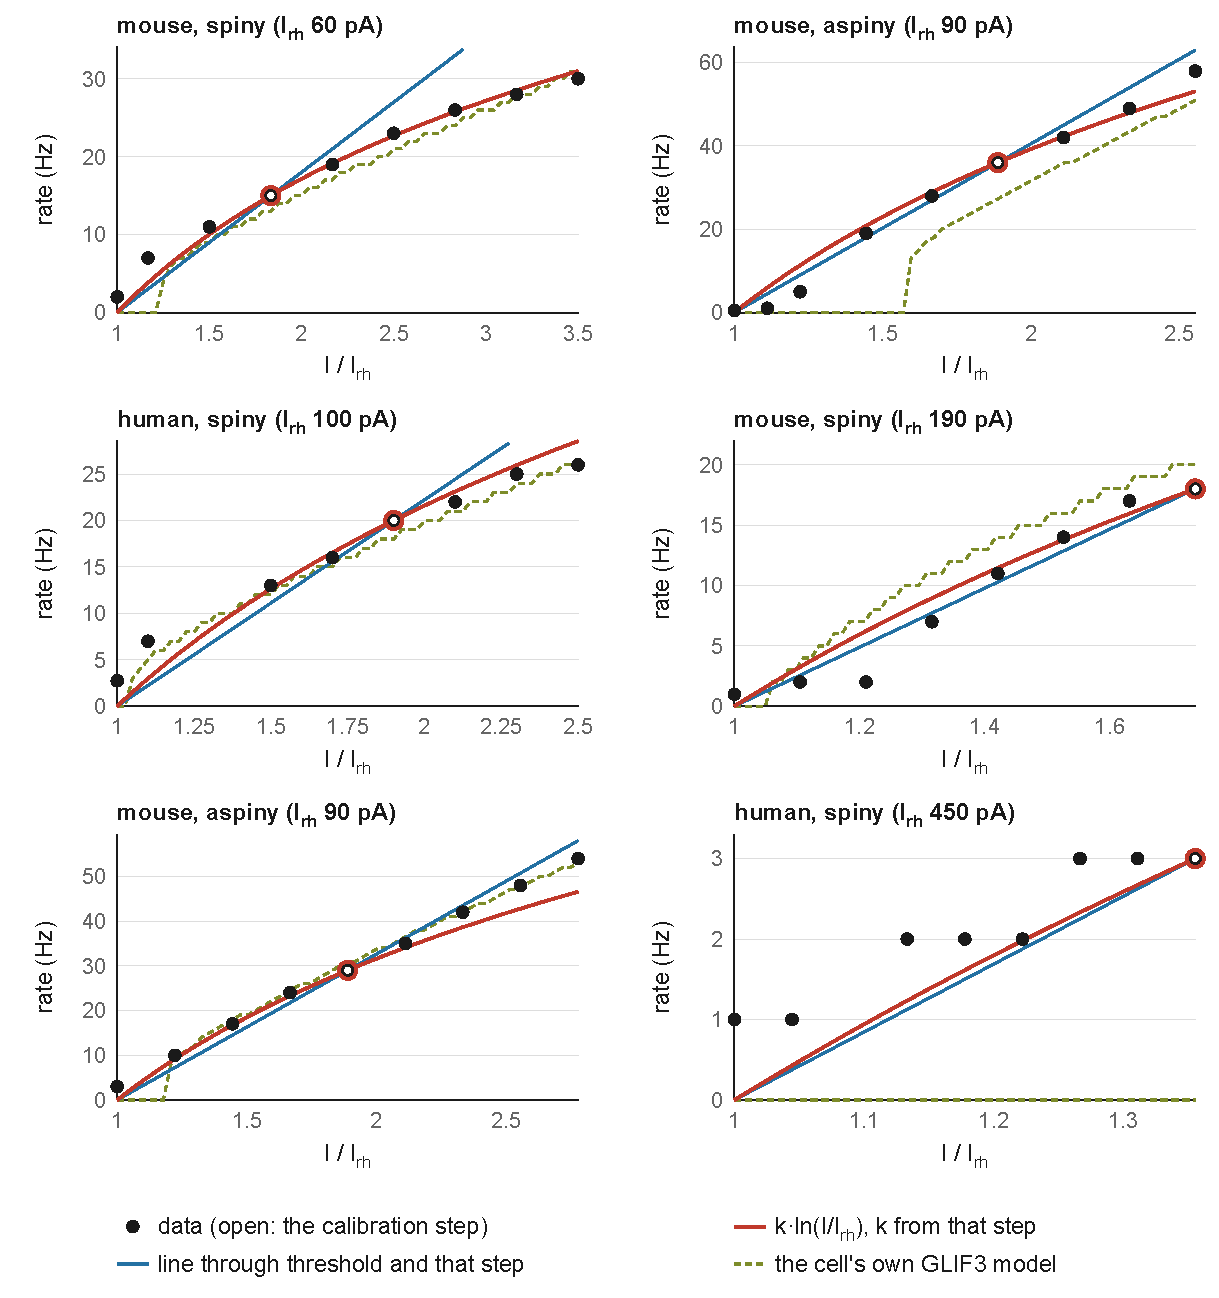
\includegraphics[width=\textwidth]{fig1_curves.pdf}
\caption{Six held-out cells: measured rates (dots; the open dot with a ring is the calibration step), the law $k\ln(I/\Irh)$ with $k$ from that step (red), the straight line through the threshold and the same step (blue), and the cell's own GLIF3 model (dashed; its rate is a spike count in a 1~s step, hence the stairs). In the last cell the model does not reach threshold at these currents. The cells are the first two, by specimen ID, of each of three groups (mouse spiny, mouse aspiny, human spiny) among the held-out cells with a GLIF3 model and at least eight steps; they illustrate and test nothing.}
\label{fig:curves}
\end{figure}

\begin{table}[htb]
\caption{The registered checks on the 588 held-out cells with at least seven suprathreshold steps. A and B: error of the predicted rates in decades, mean / median, over the steps given. C: the zero of $a + b\ln x$. D: mean absolute error of $\lgt k$.}
\label{tab:checks}
\small
\begin{tabular*}{\textwidth}{@{\extracolsep{\fill}}llll@{}}
\toprule
check & logarithmic law & comparison & result \\
\midrule
A: continuation & $a + b\ln x$ & line $a + bx$ & H1 held \\
\quad 2,047 steps & 0.123 / 0.054 & 0.131 / 0.074 & \\
\addlinespace
B: one-step calibration & $k\ln x$ & line through threshold & H2 held \\
\quad 4,447 steps & 0.209 / 0.084 & 0.225 / 0.120 & ($0.084 < 0.85 \times 0.120$) \\
\addlinespace
C: zero of the law & median $x_0$ (quartiles) & registered range & H3 held \\
\quad 582 cells & 0.987 (0.915 to 1.033) & 0.93 to 1.03 & \\
\addlinespace
D: $\lgt k$ from properties & NAI's law & log-linear regression & H4 held \\
\quad 588 cells & 0.252 & 0.273 & \\
\bottomrule
\end{tabular*}
\end{table}

\begin{table}[htb]
\caption{Check A on the held-out cells, all registered per-cell forms: the error of the 2,047 predicted rates in the upper part of each curve, in decades.}
\label{tab:forms}
\small
\begin{tabular*}{\textwidth}{@{\extracolsep{\fill}}lccc@{}}
\toprule
form & numbers per cell & mean & median \\
\midrule
line $a + bx$ & 2 & 0.131 & 0.074 \\
$a + b\sqrt{x - 1}$ & 2 & 0.171 & 0.102 \\
$a + b\ln x$ & 2 & 0.123 & 0.054 \\
$k\ln x$ & 1 & 0.124 & 0.064 \\
$a + b\ln(x - c)$ & 3 & 0.122 & 0.050 \\
$a - b\exp(-x/c)$ & 3 & 0.120 & 0.052 \\
$a + b(x - 1)^p$ & 3 & 0.143 & 0.077 \\
\bottomrule
\end{tabular*}
\end{table}

\subsection{Comparison with the cells' own GLIF models (outside the registration)}
On the 331 held-out cells with GLIF models (2,527 steps besides the calibration step), the median error was 0.078 decades for $k\ln x$ from one step, 0.118 for the line through the threshold and the same step, 0.200 for the cells' GLIF3 models and 0.301 for their GLIF1 models; the means are in Figure~\ref{fig:errors}. The 755 cells of the working part with models gave the same order (medians 0.084 for $k\ln x$ and 0.243 for GLIF3). The GLIF models were fitted to spike times under noise stimuli rather than to f--I curves, and they take no step of the curve as input, so the comparison measures how well a published model of the cell reproduces its curve, not the best a model of that kind could do.

\begin{figure}[tbp]
\centering
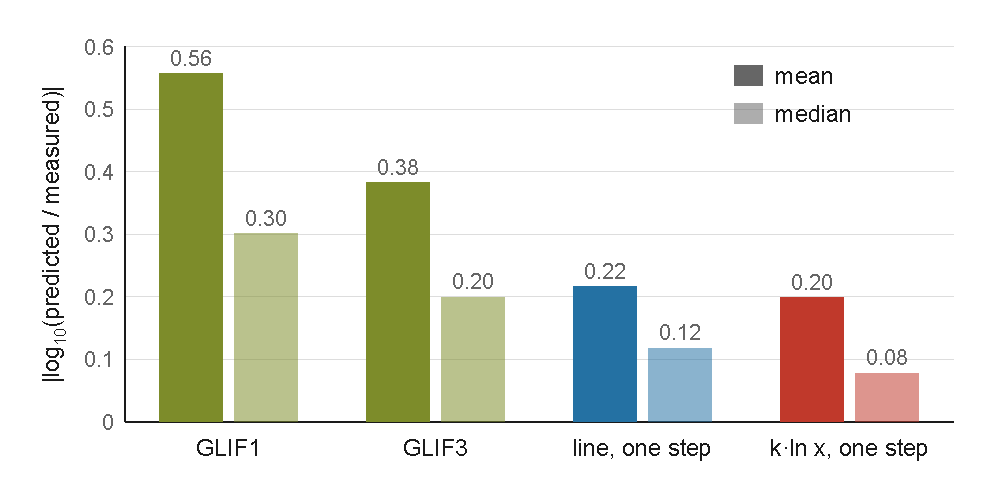
\includegraphics[width=0.8205\textwidth]{fig2_errors.pdf}
\caption{Errors of the predicted rates, $|\lgt(f_{\mathrm{pred}}/f)|$, on the 331 held-out cells with GLIF models (2,527 steps besides the calibration step). Dark bars: mean; light bars: median. Outside the registration.}
\label{fig:errors}
\end{figure}

\subsection{Scaling with the membrane time constant}
On the working part (1,340 cells), the log-linear regression of check D is
\[
\lgt k = 1.153 - 1.064\lgt\taum + 0.356\lgt R + 0.460\lgt\Irh - 0.098[\mathrm{spiny}] - 0.002[\mathrm{human}],
\]
with $k$ in Hz, $\taum$ in ms, $R$ in M$\Omega$ and $\Irh$ in pA; $[\mathrm{spiny}]$ is 1 for spiny and sparsely spiny cells and 0 for aspiny cells, $[\mathrm{human}]$ is 1 for human cells. The residual scatter is 0.36 decades. The exponent of $\taum$ is close to $-1$: $k$ scales as $1/\taum$. The dimensionless product $k\taum$ ($\taum$ in seconds) has a median of 0.53 in spiny and 0.79 in aspiny cells over all 1,928 cells (Figure~\ref{fig:tau}; 0.53 and 0.74 on the working part alone); mouse and human cells differ little (0.58 and 0.51). NAI's law for check D,
\[
\lgt k = \sqrt{2} + \tau_{\mathrm{m}}^{\,-p}\,\ln\taum, \qquad p = \taum/\sqrt{\Irh} + [\mathrm{spiny}],
\]
with $\taum$ in ms and $\Irh$ in pA, predicted the held-out cells better than the regression (Table~\ref{tab:checks}). For spiny cells it is nearly a constant, $k \approx 10^{\sqrt{2}} \approx 26$~Hz (the second term is below 0.05 for 98\,\% of them); it raises $k$ for aspiny cells with a short $\taum$. I have no mechanistic interpretation of it. Without any suprathreshold step, $k$ from the regression predicts the held-out rates above the rheobase with a median error of 0.235 decades, and $k$ from NAI's law with 0.212: one measured step is worth much more than the cell's other properties.

\begin{figure}[tbp]
\centering
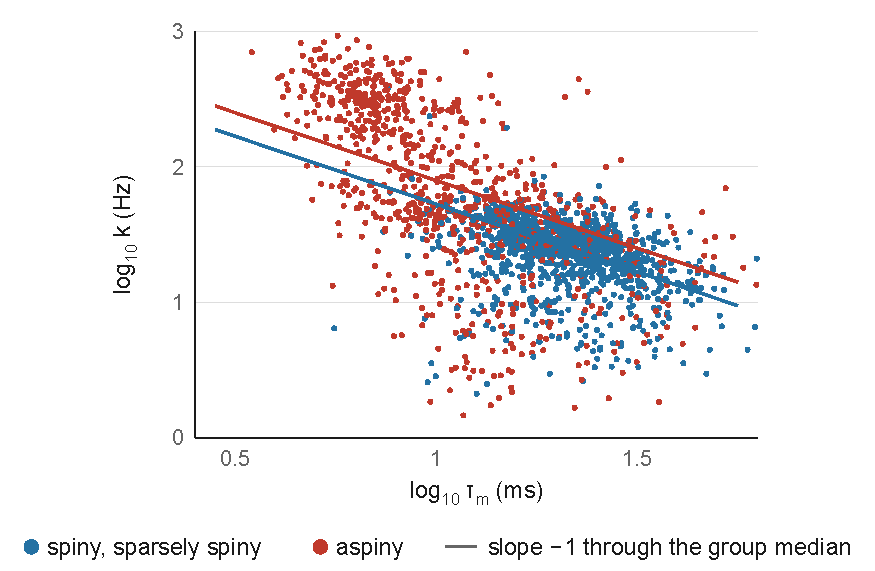
\includegraphics[width=0.7179\textwidth]{fig3_tau.pdf}
\caption{$\lgt k$ against $\lgt\taum$ for the 1,928 cells with at least seven steps (working part and held-out cells); $k$ is the least-squares fit of $k\ln x$ to the cell's curve, as in check D. The lines of slope $-1$ pass through the median of $\lgt k + \lgt\taum$ of each group. Nine cells lie outside the axes and are not shown. The pooled cloud also reflects the separation of cell types (fast-spiking interneurons have short $\taum$ and large $k$).}
\label{fig:tau}
\end{figure}

\subsection{Robustness (outside the registration)}
The one-step calibration beat the line through the threshold in every group of at least 20 cells (species, dendrite type, cortical layer), on both parts of the data: medians 0.061 to 0.114 against 0.110 to 0.155 decades. The continuation's advantage was less uniform: it vanished for human cells (median 0.061 against 0.062 on the held-out cells) and reversed for layer 3 of the working part (0.089 against 0.075).

\subsection{How logarithmic are the curves?}
I fitted $f = k(x^d - 1)/d$ to each cell with Poisson weights (variance equal to the spike count). Within $\Delta\chi^2 \le 4$ of the best $d$, the logarithm ($d = 0$) was consistent with 67\,\% of the working-part cells and 69\,\% of the held-out cells, and the line through the threshold ($d = 1$) with 57\,\% and 63\,\%. The best $d$ had a median of 0.25 and 0.40 but varied widely (quartiles $-0.9$ to 2.0 and $-0.65$ to 1.8), and for 20\,\% of the cells it lay at the edge of the searched range, $|d| = 4$, that is, it was not determined. Seven to ten steps per cell cannot separate these shapes: the one-parameter logarithm is a good compromise across cells, not the shape of each cell.

\section{Discussion}

A single number per cell, anchored at the rheobase, describes the suprathreshold f--I curves of this large and varied set of neurons well enough to be useful. The practical recipe is short: measure the rheobase $\Irh$ and one step $I_1$ near $2\Irh$, with its rate $f_1$, and take
\[
f(I) \approx f_1\,\frac{\ln(I/\Irh)}{\ln(I_1/\Irh)}, \qquad I \ge \Irh .
\]
On the held-out cells, half of the rates predicted this way were within a factor of 1.21 of the measured ones; the median error was 30\,\% lower than that of a straight line through the same two points, and lower than that of the published neuron models of the same cells. This can shorten recording protocols when only the curve is needed, and give starting values for models and network simulations.

The result has clear limits. The steps last one second, so the rates are averages over spike-frequency adaptation, and the shape of the curve may differ for other step durations or for instantaneous rates. Most curves start at the rheobase with a rate of one or a few spikes per second (median 1~Hz), so a zero of the fitted logarithm near the rheobase is close to built in, and H3 is a weak test. The scatter of $k$ between cells (0.36 decades after the regression) limits any prediction made without a suprathreshold step. The comparison with GLIF models favours a curve calibrated on the same cell over models fitted to other stimuli. The law is descriptive: it does not follow from a neuron model, and I do not propose a mechanism for it. Finally, the form is not distinguished from a straight line in most single cells; its advantage appears in prediction across many cells.

\section*{Data and code availability}
The data are from the Allen Cell Types Database (\copyright\ 2015 Allen Institute for Brain Science; available from \url{https://celltypes.brain-map.org}). The supplementary material contains the registration document and its manifest, whose SHA-256 is the fingerprint given in Section~2, the working notes and the analysis scripts as they stood at the registration (the document and the notes in their Russian originals, which the fingerprint covers, with English translations), the scripts written after it, the list of the 700 held-out cells and the numerical results. The manifest also lists the SHA-256 digests of the downloaded data and of the formula-search program. The data are not redistributed (the scripts download them from the Allen Institute's API), and the program's binary is available from the author on request.

\section*{Ethics statement}
No new data were collected. All recordings are from the public Allen Cell Types Database; the human tissue was obtained by the Allen Institute and its partner hospitals with the donors' informed consent under their approved protocols, and the database contains no information that identifies a donor.

\section*{Funding}
This work received no specific funding.

\section*{Competing interests}
I develop NAI, the formula-search program used in this work, and intend to offer it as a product and service. I declare no other competing interests.

\section*{Use of AI assistance}
The formula search was done with NAI, my own program, which uses no language model. The analysis scripts, the figures and the text of this preprint were prepared with the help of the AI assistant Claude (Anthropic). I checked the analyses and the text and take full responsibility for them.

\section*{References}
{\small
\setlength{\parindent}{0pt}
\setlength{\parskip}{4pt}
\everypar{\hangindent=1.5em \hangafter=1}
\raggedright

Allen Institute for Brain Science. Allen Cell Types Database. \url{https://celltypes.brain-map.org} (accessed 22 October 2026).

Gouwens NW, Sorensen SA, Berg J, et al.\ (2019). Classification of electrophysiological and morphological neuron types in the mouse visual cortex. \textit{Nature Neuroscience} 22:1182--1195. \href{https://doi.org/10.1038/s41593-019-0417-0}{doi:10.1038/s41593-019-0417-0}

Hodgkin AL (1948). The local electric changes associated with repetitive action in a non-medullated axon. \textit{Journal of Physiology} 107:165--181.

Roxin A, Brunel N, Hansel D, Mongillo G, van Vreeswijk C (2011). On the distribution of firing rates in networks of cortical neurons. \textit{Journal of Neuroscience} 31:16217--16226. \href{https://doi.org/10.1523/JNEUROSCI.1677-11.2011}{doi:10.1523/JNEUROSCI.1677-11.2011}

Smirnov M. NAI (No-Ansatz Inference), version 21. \url{https://naiscience.com}

Tateno T, Harsch A, Robinson HPC (2004). Threshold firing frequency--current relationships of neurons in rat somatosensory cortex: type 1 and type 2 dynamics. \textit{Journal of Neurophysiology} 92:2283--2294. \href{https://doi.org/10.1152/jn.00109.2004}{doi:10.1152/jn.00109.2004}

Teeter C, Iyer R, Menon V, et al.\ (2018). Generalized leaky integrate-and-fire models classify multiple neuron types. \textit{Nature Communications} 9:709. \href{https://doi.org/10.1038/s41467-017-02717-4}{doi:10.1038/s41467-017-02717-4}

}

\end{document}
